\begin{figure}[bp!]

  \centering
  \caption{An example of a stacked bar graph}
  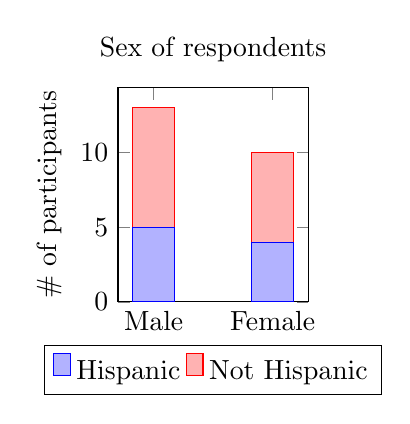
\begin{tikzpicture}
    \begin{axis}[
      title={Sex of respondents},
      ybar stacked,
      bar width=15pt,
      enlarge x limits=0.3,
      ylabel={\# of participants},
      symbolic x coords={Male,Female},
      xtick=data,
      ymin=0,
      width=4cm,
      height=4.3cm,
      legend style={at={(0.5,-0.20)},
      anchor=north,legend columns=-1},
    ]
    \addplot+[ybar] plot coordinates {(Male,5) (Female,4)};
    \addplot+[ybar] plot coordinates {(Male,8) (Female,6)};
    \legend{\strut Hispanic, \strut Not Hispanic}

    \end{axis}
  \end{tikzpicture}
\end{figure}